\chapter{\glsentrylong{GF}}

\gls{GF} is a signal processing technique for smoothing signals
(reduce high-frequency components). It is based on the convolution the
signal to filter and a Gaussian function with $\mu=0$, defined as
\begin{equation}
  g(x) = \frac{1}{\sqrt{2\pi\tau^2}}e^{-\frac{{x}^2}{2\tau^2}},
  \label{eq:GK}
\end{equation}
where $\tau$ (known as the \emph{standard deviation of the filter}
\footnote{Notice that the filter coefficients are also the values that
  a discrete random variable takes from a normal distribution.})
determines the bandwidth of the filter, and $x$ represents a distance
in the signal domain. Notice that the larger the $\tau$, the higher
the blur. In other words, $\tau$ defines the bandwidth of the filter.

In the signal domain, \gls{GF} is described as
\begin{equation}
  \text{GF}(\mathbf{s}) = \mathbf{s}\ast\mathbf{g},
\end{equation}
where $\mathbf{g}$ is a Gaussian kernel.

\section{Separability}
Multidimensional \gls{GF} is separable (see
Appendix~\ref{sec:GF_separability}), which means that we can apply the
1D filter to the $D$ dimensions of the signal to compute a $D$D
denoising. De facto, Gaussian kernels are the only circularly
symmetric kernels that are also separable
\cite{gonzalez1992digital}. For example, in the 3D case (see
Fig.~\ref{fig:3D_GF}), we have that
\begin{equation}
  \tilde{\mathbf{s}} = \Big(\big(\hat{\mathbf s}*^{(\text{Z})}{\mathbf g}\big)*^{(\text{Y})}{\mathbf g}\Big)*^{(\text{X})}{\mathbf g},
    \label{eq:3D_GF}
\end{equation}
where ${\mathbf s}*^{(d)}{\mathbf g}$ is the 1D convolution applied to
the dimension $d$ of the signal ${\mathbf s}$ and the (1D) kernel
${\mathbf g}$. For simplicity, Eq.~\ref{eq:3D_GF} defines isotropic
filtering, but $\tau$ can be different at each dimension to provide
anisotropy. Eq.~\ref{eq:3D_GF} is implemented
\href{https://github.com/vicente-gonzalez-ruiz/denoising/blob/main/src/denoising/volume/gaussian.py}{here},
and the corresponding 2D version is implemented
\href{https://github.com/vicente-gonzalez-ruiz/denoising/blob/main/src/denoising/image/gaussian.py}{here}.

Separability increases speed. For example, a 1D \gls{GF} horizontally
and then vertically (or vice versa) instead of doing a 2D convolution,
which is faster than a 2D convolution. The speed-up provied by
separability in this (2D case) is (in terms of \gls{NoO})
\begin{equation}
  \text{Speed-up} = \frac{\text{NoO~in~the~2D-convolution}}{\text{NoO~in~1D-convolution~of~the~rows}+\text{NoO~in~1D-convolution~of~the~columns}} = \frac{MNK^2}{2MNK} = \frac{K}{2},
\end{equation}
where $M$ and $N$ are the width and height of the filtered image, and
$K$ is the length of the Gaussian kernel.

\section{Denoising using \acrshort{GF}}
%{{{

Gaussian kerners are low-pass filters\footnote{We can distinguish this
  because all the coefficients of the kernel are positive numbers.},
and the \gls{SNR} is usually smaller in the high
frequencies. Therefore, when we filter a noisy signal using \gls{GF}
what we are basically eliminating is noise.

On the other hand, unlike other digital filters, such as an ideal low-pass
filter, a Gaussian low-pass filter does not generate ringing (the
transfer function of a Gaussian filter is another Gaussian filter,
which does not have lobes), and the convolution of two Gaussians are Gaussian
functions as well. 

In \gls{GD} we have that
\begin{equation}
  \tilde{\mathbf{s}} = \hat{\mathbf{s}}\ast\mathbf{g},
  \label{eq:GF}
\end{equation}
where $\tilde{\mathbf{s}}$ represents the denoised signal, $\hat{\mathbf{s}}$ the noisy signal, and $\mathbf{g}$ the Gaussian kernel.

\begin{figure}
  \centering
  \includegraphics[width=0.8\textwidth]{3D_GF}
  \caption{3D Gaussian filtering. The gray planes contain the voxels
    that are filtered and the white planes contain the voxels used by
    the 1D kernel when it is applied to the voxels of the filtered
    plane. The kernel shown here contains 3 coefficients. The volume
    is convolved sequentially in-place, from left to
    right.\label{fig:3D_GF}}
\end{figure}


\begin{comment}
%{{{

 This idea has been describen in Python pseudo-code in
the Fig.~\ref{fig:3DGF_imple}.

\begin{figure}
\noindent $\mathsf{3DGF}(\hat{\mathbf{X}}, \mathbf{h})$: $\rightarrow\tilde{\mathbf{X}}$
\vspace{-1ex}
\begin{enumerate}
  \setlength{\itemsep}{0pt}
\item [1.] $\tilde{\mathbf{X}}\leftarrow\href{https://docs.opencv.org/2.4/modules/imgproc/doc/geometric_transformations.html#resize}{\mathsf{resize}}(\hat{\mathbf{X}}, \mathsf{dsize}=)$
\item [2.] $\mathsf{for}~z~\mathsf{in}~\mathsf{range}(\hat{\textbf{X}}.\mathsf{shape}_0),~\mathsf{run}$:  \hfill $\mathtt{/*~Filtering~in~the~Z~direction~*/}$
  \begin{enumerate}
  \item [1.] $\mathsf{for}~h~\mathsf{in~range}(\mathbf{h}.\mathsf{size})$:
    \begin{enumerate}
    \item [1.] $\tilde{\mathbf{X}}_{z,:,:}\leftarrow\tilde{\mathbf{X}}_{z,:,:}+\hat{\mathbf{X}}_{z,:,:}\mathbf{h}_{h}$
    \end{enumerate}
  \end{enumerate}
\item [3.] $\mathsf{for}~y~\mathsf{in}~\mathsf{range}(\hat{\textbf{X}}.\mathsf{shape}_1),~\mathsf{run}$:  \hfill $\mathtt{/*~Filtering~in~the~Y~direction~*/}$
  \begin{enumerate}
  \item [1.] $\mathsf{for}~k~\mathsf{in~range}(\mathbf{h}.\mathsf{size})$:
    \begin{enumerate}
    \item [1.] $\tilde{\mathbf{X}}_{:,y,:}\leftarrow\tilde{\mathbf{X}}_{:,y,:}+\hat{\mathbf{X}}_{:,y,:}\mathbf{h}_{h}$
    \end{enumerate}
  \end{enumerate}
\item [4.] $\mathsf{for}~x~\mathsf{in}~\mathsf{range}(\hat{\textbf{X}}.\mathsf{shape}_2),~\mathsf{run}$:  \hfill $\mathtt{/*~Filtering~in~the~X~direction~*/}$
  \begin{enumerate}
  \item [1.] $\mathsf{for}~h~\mathsf{in~range}(\mathbf{h}.\mathsf{size})$:
    \begin{enumerate}
    \item [1.] $\tilde{\mathbf{X}}_{:,:,x}\leftarrow\tilde{\mathbf{X}}_{:,:,x}+\hat{\mathbf{X}}_{:,:,x}\mathbf{h}_{h}$
    \end{enumerate}
  \end{enumerate}
\end{enumerate}
%\end{myquote}
\caption{Python pseudo-code of 3DGF using periodic signal extension.}
\label{fig:3DGF_imple}
\end{figure}

%}}}
\end{comment}

\begin{figure}
  \centering
  \resizebox{1.0\textwidth}{!}{
    \renewcommand{\arraystretch}{0.0} % Adjust row spacing in the table
    \setlength{\tabcolsep}{0ex}      % Adjust column spacing in the table    
    \begin{tabular}{cc}
      %\href{https://nbviewer.org/github/vicente-gonzalez-ruiz/denoising/blob/main/notebooks/barb.ipynb}{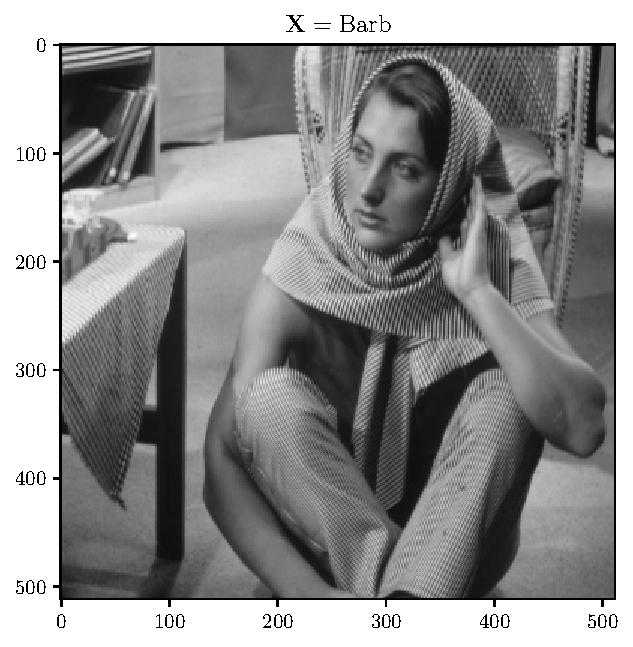
\includegraphics{barb}} & \href{https://nbviewer.org/github/vicente-gonzalez-ruiz/denoising/blob/main/figs/lake.ipynb}{\includegraphics{lake}} \\
      %\href{https://nbviewer.org/github/vicente-gonzalez-ruiz/denoising/blob/main/notebooks/barb_0MMPG.ipynb}{\includegraphics{barb_0MMPG}} & \href{https://nbviewer.org/github/vicente-gonzalez-ruiz/denoising/blob/main/notebooks/lake_0MMPG.ipynb}{\includegraphics{lake_0MMPG}} \\
      \href{https://nbviewer.org/github/vicente-gonzalez-ruiz/denoising/blob/main/notebooks/Confocal_FISH_GF_optimal_tau.ipynb\#Confocal_FISH_GF_optimal_tau}{\includegraphics{Confocal_FISH_GF_optimal_tau.pdf}} & \href{https://nbviewer.org/github/vicente-gonzalez-ruiz/denoising/blob/main/notebooks/TwoPhoton_MICE_GF_optimal_tau.ipynb\#TwoPhoton_MICE_GF_optimal_tau}{\includegraphics{TwoPhoton_MICE_GF_optimal_tau.pdf}}
    \end{tabular}
  }
  \caption{Optimal $\tau$ values in GF. These curves have been
    determined by filtering images with different levels of
    (artificial, see Eq,~\ref{eq:MPG_noise_model}) MPG noise and
    comparing (see Eq.~\ref{eq:PCC}) the result with the
    \gls{GT}.\label{fig:optimal_GF_tau}}
\end{figure}

As can be seen in Eq.~\ref{eq:GK}, the denoising result depends on
$\tau$. An optimal value for the standard deviation of the kernel,
$\tau^*$, can be found if $\mathbf{s}$ were known(see
Fig.~\ref{fig:optimal_GF_tau}). Unfortunately, $\mathbf{s}$ is usually
unknown and we only can estimate $\tau^*$. Ideally, $\tau^*$ should
increase the \gls{SNR} as much as possible, considering also that: (1)
\gls{GF} attenuates the high frequencies, (2) the \gls{SFC} of the
noise is close to zero, and (3) that most of the energy (information)
in the signals are concentrated in the low frequencies. Therefore, we
should find a cut-off frequency
\begin{equation}
  \eta^* = \text{min}\{\eta|\text{SFC}(\hat{\mathbf{s}})_\eta < \alpha\},
  \label{eq:search_eta}
\end{equation}
where $\alpha$ is the minimun correlation that should reach the SFC to consider that the corresponding ring/shell has a high enough \gls{SNR} (see
Appendix~\ref{sec:tau_VS_eta}). Once we have already estimated
$\eta^*$, we can use the corresponding $\tau^*$ to filter out those
frequency components of $\hat{\mathbf{s}}$ with the lowest SNR.

\begin{figure}
  \centering
  \resizebox{1.0\textwidth}{!}{
    \renewcommand{\arraystretch}{0.0} % Adjust row spacing in the table
    \setlength{\tabcolsep}{0ex}      % Adjust column spacing in the table    
    \begin{tabular}{cc}
      \href{https://nbviewer.org/github/vicente-gonzalez-ruiz/denoising/blob/main/notebooks/Confocal_FISH_GF_estimation.ipynb}{\includegraphics{Confocal_FISH_GF_estimation.pdf}} & \href{https://nbviewer.org/github/vicente-gonzalez-ruiz/denoising/blob/main/notebooks/TwoPhoton_MICE_GF_estimation.ipynb}{\includegraphics{TwoPhoton_MICE_GF_estimation.pdf}}
    \end{tabular}
  }
  \caption{Optimal VS estimated $\tau^*$ values.\label{fig:tau_GF_estimation}}
\end{figure}

In the Fig.~\ref{fig:tau_GF_estimation} there is a comparison between
the true $\tau^*$ values and their estimations, using the \gls{EOS}
technique (see Appendix~\ref{sec:EOS}) to compute the \gls{SFC} curves (see
Section~\ref{sec:fourier_correlation}). Specifically, we have used
(see Eq.~\ref{eq:ideal_hat_tau} and Fig.~\ref{fig:eta_vs_tau})
\begin{equation}
  \tau^*_{\text{EOS}} = \frac{0.141}{2\eta^*},
  \label{eq:tau_VS_eta_empirical_EOS}
\end{equation}
(and not exactly the fitting expression approximated in the
Fig.~\ref{fig:eta_vs_tau}) because using signal splitting to compute
the \gls{SFC}, only the first half of the frequencies provide reliable
information. Notice that, to determine $\eta^*$ (the estimated
``optimal'' cut-off frequency of the Gaussian filter) we have assumed
that an attenuation higher than $1/\sqrt{2}$ (see
Appendix~\ref{sec:tau_VS_eta}) can be high enought to remove the
frequencies higher than $\eta^*$.

%Appendix~\ref{sec:results} contains a table with the performance of some denoisers.

%{\color{red} Podemos comparar diferentes algoritmos de denoising si usamos, para una determinada configuración de ruido, el filtrado óptimo (que es posible encontrar porque tenemos el GT). Nos va a salir una tabla con valores de PCC.}

%Since all denoising algorithms have a similar behavior (they tend to
%eliminate high frequencies and preserve low ones), we will consider
%Eq.~\ref{eq:tau_VS_eta_empirical_EOS} as generic and it will be used
%to find the optimal value of the different operating parameters of the
%denoising algorithms.

\begin{comment}
\begin{figure}
  \centering
  \resizebox{1.0\textwidth}{!}{
    \renewcommand{\arraystretch}{0.0} % Adjust row spacing in the table
    \setlength{\tabcolsep}{0ex}      % Adjust column spacing in the table    
    \begin{tabular}{cc}
      \href{https://nbviewer.org/github/vicente-gonzalez-ruiz/denoising/blob/main/notebooks/barb.ipynb}{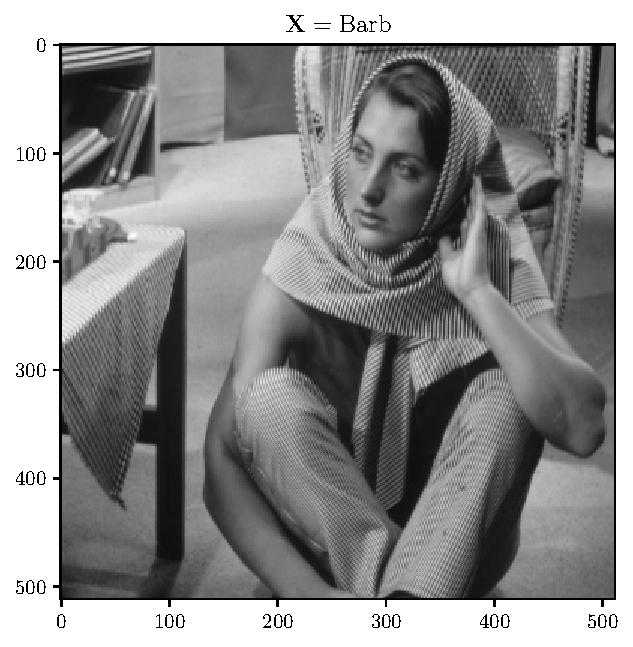
\includegraphics{barb}} & \href{https://nbviewer.org/github/vicente-gonzalez-ruiz/denoising/blob/main/figs/lake.ipynb}{\includegraphics{lake}} \\
      \href{https://nbviewer.org/github/vicente-gonzalez-ruiz/denoising/blob/main/notebooks/tau_VS_img.ipynb\#0MMPG_barb}{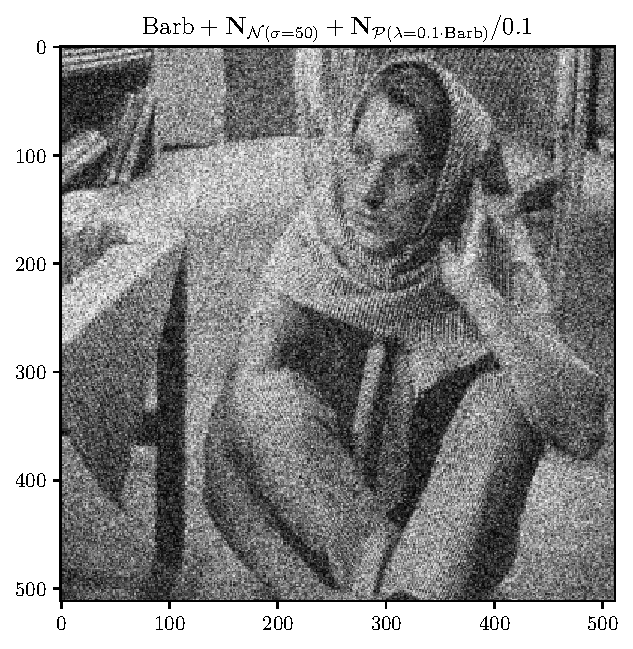
\includegraphics{0MMPG_barb}} & \href{https://nbviewer.org/github/vicente-gonzalez-ruiz/denoising/blob/main/figs/tau_VS_img.ipynb\#0MMPG_lake}{\includegraphics{0MMPG_lake}} \\
      \href{https://nbviewer.org/github/vicente-gonzalez-ruiz/denoising/blob/main/notebooks/tau_VS_img.ipynb\#GF_0MMPG_barb}{\includegraphics{GF_0MMPG_barb}} & \href{https://nbviewer.org/github/vicente-gonzalez-ruiz/denoising/blob/main/figs/tau_VS_img.ipynb\#GF_0MMPG_lake}{\includegraphics{GF_0MMPG_lake}}
    \end{tabular}
  }
  \caption{Two examples of optimal denoising using GF. On the top, the
    original images. In the middle, the noisy instances. On the
    bottom, the denoised images. {\color{red} arreglar PSNRs y elegir
      tau optimo para ejemplo}\label{fig:GF_tau_optimal}}
\end{figure}
\end{comment}

\begin{figure}
  \centering
  \resizebox{1.0\textwidth}{!}{
    \renewcommand{\arraystretch}{0.0} % Adjust row spacing in the table
    \setlength{\tabcolsep}{0ex}      % Adjust column spacing in the table    
    \begin{tabular}{cc}
      Confocal\_FISH & TwoPhton\_MICE \\
      \href{https://nbviewer.org/github/vicente-gonzalez-ruiz/denoising/blob/main/notebooks/Confocal_FISH_noisy__GF.ipynb}{\includegraphics{Confocal_FISH_noisy}} & \href{https://nbviewer.org/github/vicente-gonzalez-ruiz/denoising/blob/main//notebooks/TwoPhoton_MICE_noisy__GF.ipynb}{\includegraphics{TwoPhoton_MICE_noisy}} \\
      \href{https://nbviewer.org/github/vicente-gonzalez-ruiz/denoising/blob/main/notebooks/Confocal_FISH_noisy__GF.ipynb}{\includegraphics{Confocal_FISH_denoised__GD}} & \href{https://nbviewer.org/github/vicente-gonzalez-ruiz/denoising/blob/main/notebooks/TwoPhoton_MICE_noisy__GF.ipynb}{\includegraphics{TwoPhoton_MICE_denoised__GD}}
    \end{tabular}
  }
  \caption{Two examples of \emph{optimized} denoising using \gls{GD}
    ($\tau^*$ has been selected using the algorithm described in the
    text). On the top, the noisy instances (the \glspl{GT} are in the
    Appendix~\ref{sec:images}). At the bottom, the denoised
    versions.\label{fig:optimal_GD}}
\end{figure}

\begin{comment}
%{{{

Concretelly, we use (see
Appendix~\ref{SFC_random_data})
\begin{equation}
  \tau^*_{\text{SPRS}} = \frac{0.141}{5(\eta^*-0.09)},
  \label{eq:tau_VS_eta_empirical_SPRS}
\end{equation}
when we are using the SPRS algorithm to find the SFC curve, or
\begin{equation}
  \tau^*_{\text{EO}} = \frac{0.141}{3(\eta^*-0.01)},
  \label{eq:tau_VS_eta_empirical_EO}
\end{equation}
if we are using the EO algorithm to find the SFC curve,
where we are supposing that $\beta=1/\sqrt{2}$ (see
Appendix~\ref{sec:tau_VS_eta}). 

Fig.~\ref{fig:tau_GF_estimation} shows the result of using
Eqs.~\ref{eq:tau_VS_eta_empirical_SPRS} and
\ref{eq:tau_VS_eta_empirical_EO} for estimating $\tau^*$ for the two
test images. As can be seen ..

%}}}
\end{comment}

\begin{comment}
%{{{

Assuming that most of the signal energy (information) is concentrated
in the low frequencies, higher values of $\tau$ will produce a higher
smoothing effect in $\tilde{\mathbf{X}}$). More concretely, if
$\mathcal{F}(h)=H$, that is
\begin{equation}
  H(u) = e^{-\frac{u^2}{2\tau^{-2}}},
\end{equation}
it can be seen that if $\tau$ increases, the cut-off frequency
provided by $H$ decreases, and viceversa. 


\begin{figure}
  \centering
  \resizebox{1.0\textwidth}{!}{
    \renewcommand{\arraystretch}{0.0} % Adjust row spacing in the table
    \setlength{\tabcolsep}{0ex}      % Adjust column spacing in the table    
    \begin{tabular}{cc}
      \href{https://nbviewer.org/github/vicente-gonzalez-ruiz/denoising/blob/main/notebooks/barb.ipynb}{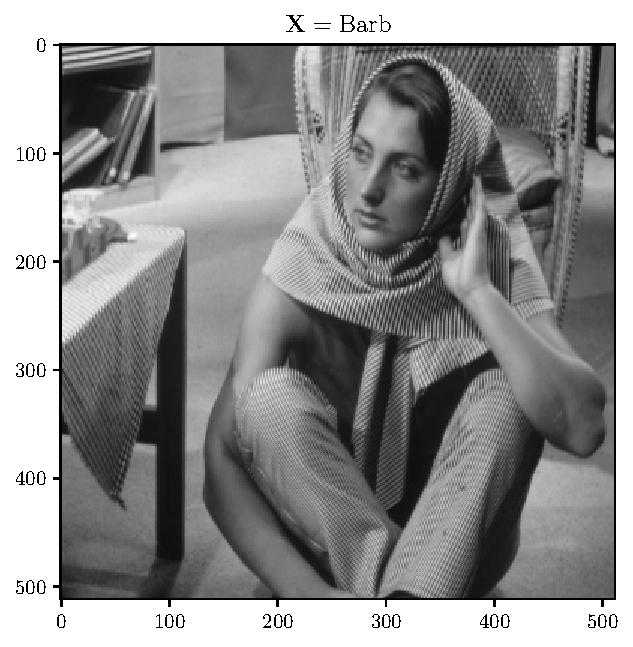
\includegraphics{barb}} & \href{https://nbviewer.org/github/vicente-gonzalez-ruiz/denoising/blob/main/figs/lake.ipynb}{\includegraphics{lake}} \\
      \href{https://nbviewer.org/github/vicente-gonzalez-ruiz/denoising/blob/main/notebooks/tau_VS_img.ipynb\#0MMPG_barb}{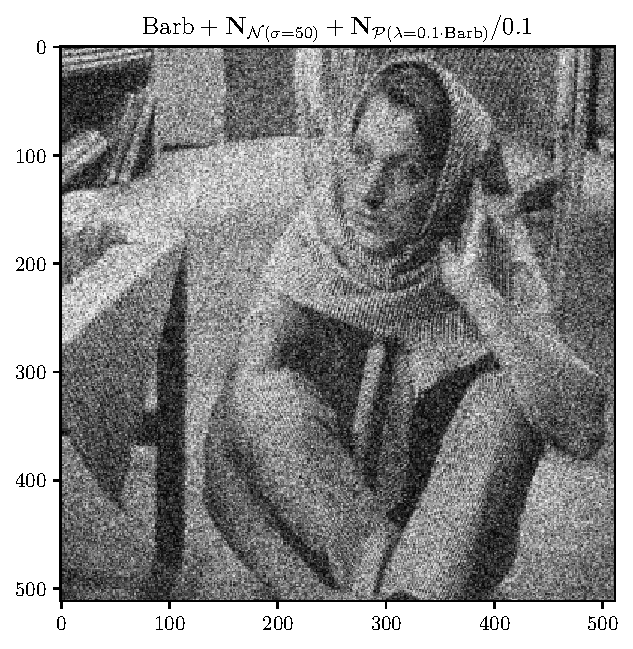
\includegraphics{0MMPG_barb}} & \href{https://nbviewer.org/github/vicente-gonzalez-ruiz/denoising/blob/main/figs/tau_VS_img.ipynb\#0MMPG_lake}{\includegraphics{0MMPG_lake}} \\
      \href{https://nbviewer.org/github/vicente-gonzalez-ruiz/denoising/blob/main/notebooks/tau_VS_img.ipynb\#GF_0MMPG_barb}{\includegraphics{GF_0MMPG_barb}} & \href{https://nbviewer.org/github/vicente-gonzalez-ruiz/denoising/blob/main/figs/tau_VS_img.ipynb\#GF_0MMPG_lake}{\includegraphics{GF_0MMPG_lake}}
    \end{tabular}
  }
  \caption{Two examples of optimal denoising using GF. On the top, the
    original images. In the middle, the noisy instances. On the
    bottom, the denoised images. {\color{red} arreglar PSNRs y elegir
      tau optimo para ejemplo}\label{fig:GF_tau_optimal}}
\end{figure}

Fig.~\ref{fig:tau_VS_image} shows the denoising performance of GF for
two artificially noised images, for different levels of noise
($\sigma$) and filter length ($\tau$). As can be seen, the optimal
value of the filter length, $\tau^*$ (which maximizes the PCC between
$\mathbf{X}$ and $\tilde{\mathbf{X}}$), depends on the noise level and
$\mathbf{X}$, information that is, in general, unavailable in
microscopy imaging. Therefore, $\tau^*$ can be only
\emph{estimated}\footnote{Notice that, only knowing $\mathbf{X}$ it
  would be possible to find $\tau^*$. Therefore, the furthest one can
  go is to estimate the optimal filtering parameters}. depending on,
for example, the (subjective) visual quality of
$\tilde{\mathbf{X}}$. An example of optimal denoising using GF has
been show in Fig.~\ref{fig:GF_tau_optimal}.

% \begin{figure}
%   \centering
%   \resizebox{1.0\textwidth}{!}{
%     \renewcommand{\arraystretch}{0.0} % Adjust row spacing in the table
%     \setlength{\tabcolsep}{0ex}      % Adjust column spacing in the table    
%     \begin{tabular}{cc}
%   \href{https://nbviewer.org/github/vicente-gonzalez-ruiz/denoising/blob/main/figs/gaussian_denoising.ipynb\#GD_SFRC_0MMPG_NL20_barb}{\includegraphics{GD_SFRC_0MMPG_NL20_barb}} & \href{https://nbviewer.org/github/vicente-gonzalez-ruiz/denoising/blob/main/figs/gaussian_denoising.ipynb\#GD_SFRC_0MMPG_NL60_barb}{\includegraphics{GD_SFRC_0MMPG_NL60_barb}}
%     \end{tabular}
%     }
%     \caption{SFRC curves for two different noisy instances of
%       Barb, see Fig.~\ref{fig:tau_VS_image} using two
%       different noise levels ($\sigma=20$ and $\sigma=60$), and after
%       having applied GD for several filter lengths. As can be seen, for $\sigma=20$, the ``optimal'' filter
%       length (that maximizes the area below the curve) is ..., and for
%       $\sigma=60$, the ``optimal'' filter length is ... Therefore, the
%       ``optimal'' filter length is (positively) correlated with the
%       noise level. Notice that $\tau$
%       has been discretized in steps of $0.25$.

%       (2) the
%       ``optimal'' filter length is (positively) correlated with the
%       noise level (for the noise level $\sigma=40$ and $\gamma=0.15$
%       the ``optimal'' $\tau=1.0$ and the noise level $\sigma=50$ and
%       $\gamma=0.15$ the ``optimal'' $\tau=1.25$). Notice that $\tau$
%       has been discretized in steps of $0.25$.


%       Relation between the SFRC curves and the filter length of
%       a Gaussian filter. $\hat{\mathbf{X}}_1$ is the the noise image
%       (Barb) shown in the Fig.~\ref{fig:tau_VS_image} (for $\sigma=40$
%       and $\gamma=0.15$). As can be seen, the area below the curve is
%       maximized for $\tau=1.0$

%       Effect of zero-mean MPG noise in an image and how GD
%     can be used to reduce it. A noisy version of the
%     image is on the top-left. On the top-right, the SFRC curves
%     of the denoised image for different filter lengths. As can be seen
%     in this subfigure, for the noise level
%     $(\sigma=40, \gamma=0.15)$, an optimal $\tau=1.25$ should be used if
%     (considering that the area below the SFRC curve should be maximized).
%     On the bottom-left, it can be seen that for this noise level,
%     the ``optimal'' Gaussian kernel-lenght is $\tau/2=0.625 \approx 0.7$. The resulting
%     ``optimal'' filtered image (using GD) is shown on the bottom-right.
%     \label{fig:GD_0MMPG}}
% \end{figure}

{\color{red} ------ comienzo sin terminar ------ }

It is also possible to estimate $\tau^*$ using the self-correlation in
the Fourier domain \cite{koho2019fourier} {\color{red}Este sería un
  buen punto para hablar de cómo estamos calculando la curva
  SF{R|S}C}. The idea here is to determine the frequency $u^*$ for
which, to the right of this frequency, the SNR decays under some given
threshold.

A more objective procedure to estimate $\tau^*$ should be based on
some (objective) quality metric, such as the self-correlation in the
Fourier domain \cite{koho2019fourier}. Fig.~\ref{fig:GD_0MMPG} shows
the result of using the SFRC of the noisy image to estimate $\tau^*$,
considering the idea that the low-pass filter should remove those
frequency components where the SNR is lower than a given threshold.



Fig.~\ref{fig:GD_0MMPG} shows
SFRC curves for different filter lengths, and it has been also
computed the normalized area below each curve, a metric that is
(positively) correlated with $\tau^*$ (see
Fig.~\ref{fig:tau_VS_image}). As can be seen that, $\tau^*$ can be
estimated using the filter length that maximizes the area below the
corresponding SFRC curve.


because the
higher the area, the higher also the PCC between the Fourier
coefficients


and it can be seen, the normalized area below the curve can be used to estimate


Another alternative can use some heuristic to estimate

We propose a more automatic procedure to find $\tau^*$.  by maximizing
the ratio between the amount of noise and the amount of signal removed
by the filter. To determine this, we can use the SFRC curve (see
Sec.~\ref{sec:FSC}), in which each point represents the correlation
between two\footnote{Actually, each point is the average (arithmetic
  mean) of two correlation coefficients, each one obtained after
  subsampling the image in each dimension (by rows, and by columns).}
rings of Fourier coefficients, extracted from two subsampled versions
of $\tilde{\mathbf{X}}$.

for the single parameter that GD requires (the length of
the Gaussian kernels in each dimension, represented by $\tau$ in
$\mathrm{GD}_\tau$) depends on the noise level, an information that is
generally unknown in microscopy imaging.

To estimate the relation between the filter length that should
maximize the quality of the denoised signal, the SFRC (Self Fourier
Ring Correlation, see Section~\ref{sec:FSC}) of several noisy
instances of the same image (variying the level of noise) has been
shown in the Fig.~\ref{fig:SFRC}.

has been calculated by subbands of a filtered
image, generating a number of SFRC curves, one for each different
kernel length $\tau$ (see Fig.  \ref{fig:GD_0MMPG}). As can be seen,
the autocorrelation increases when the noise level decreases due to
increasing $\tau$, until it reaches a value for which the
autocorrelation decreases again\footnote{Remember that the SFRC metric
  quantifies the correlation between subsampled versions of the same
  input signal and that, by definition, the MPG noise should be
  uncorrelated. For this reason, if noise were only had at the input,
  we should obtain a flat SFRC that approximates to zero. Therefore,
  the higher the area below the SFRC curve, the higher the presence of
  signal.}. For that $\tau^*$, which maximizes the area under the
curve up to the normalized frequency $\omega/4$, is when the PCC
metric is also maximized (considering the original image resolution,
i.e., without the subsampling required to compute the SFRC) for
$\tau^*/2$, which means that we can use the SFRC metric (in the 2D
case) and the SFSC (in the 3D case) to estimate the optimal filtering
parameters knowing only the noisy instance $\hat{\mathbf{X}}$.

{\color{red} ------ fin sin terminar ------ }

%}}}
\end{comment}

%}}}

\begin{subappendices}

\section{Fourier transform of a Gaussian function}
\label{sec:FTGF}
%{{{

Let the Gaussian function defined by
\begin{equation}
  h(x) = \frac{1}{\sqrt{2\pi}\tau}e^{-\frac{{x}^2}{(2\tau^2)}},
  \label{eq:gaussian_ape}
\end{equation}
(see Eq.~\ref{eq:GF}), the Fourier transform  is
\begin{equation}
  H(w) = \mathcal{F}\{h(x)\} = \int_{-\infty}^{\infty}h(x)e^{-jwx}dx,
\end{equation}
where
\begin{equation}
  w = 2\pi f,
\end{equation}
representing $f$ frequency (in the case of working with images, in
cycles per pixel-size measured in units of distance, or simply, cycles
per sample) and $w$ angular frequency (radians per unit distance, or
simply, radians per sample). Therefore,
\begin{equation*}
  H(w) = \int_{-\infty}^{\infty}\frac{1}{\sqrt{2\pi}\tau}e^{-\frac{x^2}{2\tau^2}}e^{-jwx}dx = 
\end{equation*}
\begin{equation*}
  \frac{1}{\sqrt{2\pi}\tau}\int_{-\infty}^{\infty}e^{-\frac{x^2}{2\tau^2}}e^{-jwx}dx = 
\end{equation*}
\begin{equation*}
  \frac{1}{\sqrt{2\pi}\tau}\int_{-\infty}^{\infty}e^{-\frac{x^2}{2\tau^2}-jwx}dx.
\end{equation*}
Operating in the exponent
\begin{equation*}
  -\frac{x^2}{2\tau^2}-jwx = -\frac{1}{2\tau^2}(x+2j\tau^2wx)
\end{equation*}
that after adding and subtracting $(j\tau^2w)^2$
\begin{equation*}
  = \frac{1}{2\tau^2}[(x+j\tau^2w)^2-(j\tau^2w)^2]
\end{equation*}
and rewriting and operating
\begin{equation*}
  = -\frac{(x+j\tau^2w)^2}{2\tau^2} + \frac{\tau^2w^2}{2}.
\end{equation*}
Replacing the exponent,
\begin{equation*}
  H(w) = \frac{1}{\sqrt{2\pi}\tau}e^{-\frac{\tau^2w^2}{2}}\int_{-\infty}^{\infty}e^{-\frac{(x+j\tau^2w)^2}{2\tau^2}}dx.
\end{equation*}
Now define
\begin{equation*}
  u = x + j\tau^2w.
\end{equation*}
Therefore,
\begin{equation*}
  H(w) = \frac{1}{\sqrt{2\pi}\tau}e^{-\frac{\tau^2w^2}{2}}\int_{-\infty}^{\infty}e^{{-u^2}{2\tau^2}}du.
\end{equation*}
The remaining integral is a standard Gaussian integral,
\begin{equation*}
  \int_{-\infty}^{\infty}e^{{-u^2}{2\tau^2}}du = \sqrt{2\pi}\tau.
\end{equation*}
Finally, we obtain that
\begin{equation}
  H(w) = e^{-\frac{\tau^2w^2}{2}},
  \label{eq:FTGF}
\end{equation}
that corresponds to the transfer function (i.e., the response of
Eq.~\ref{eq:gaussian_ape} to the impulse signal) of the Gaussian.

%}}}

\section{Cut-off frequency of a Gaussian filter}
\label{sec:tau_VS_eta}
%{{{

Gaussian filters are low-pass filters. In a low-pass filter we can
distinguish three subbands: (1) the pass-band, that is defined by
those range of frequencies that are not attenuated significantly, (2)
the stop-band, where the frequencies are attenuated (significantly),
and (3) the transition-band, defined by those frequencies that are not
included in the previous subbands. Notice that only in an ideal
filter, the size of the transition-band is zero.

The cut-off frequency of a low-pass filter is defined by those
frequencies of the transition-band where the response (or gain) of the
filter decreases by some given factor $\beta\in]0,1[$. In other words,
if $H$ is the transfer function of the filter,
\begin{equation}
  H(\eta) = \beta,
\end{equation}
where $\eta$ is the cut-off frequency. In the case of a Gaussian
filter (see Eq.~\ref{eq:FTGF}), we have that
\begin{equation*}
  H(\eta) = e^{-\frac{\tau^2\eta^2}{2}} = \beta.
\end{equation*}
Taking the natural logarithm
\begin{equation*}
  -\frac{\tau^2\eta^2}{2} = \ln\beta.
\end{equation*}
Solving for $\tau$
\begin{equation}
  \tau = \frac{\sqrt{-2\ln\beta}}{\eta}.
  \label{eq:tau_VS_eta}
\end{equation}

Typically, $\beta=1/\sqrt{2}$ that is equivalent to attenuate the
input signal in -3dB. Notice that at the frequency 0 (see
Eq.~\ref{eq:FTGF}),
\begin{equation*}
  H(0) = e^0=1.
\end{equation*}

Eq.~\ref{eq:tau_VS_eta} uses angular frequency. We can obtain the
corresponding expresión for ``standard'' frequency, knowing that
\begin{equation}
  \eta = 2\pi\hat{\eta}.
  \label{eq:eta_freq}
\end{equation}
Using Eq.~\ref{eq:eta_freq} into Eq.~\ref{eq:tau_VS_eta}, we obtain
\begin{equation}
  \tau = \frac{\sqrt{-2\ln\beta}}{2\pi\hat{\eta}}.
  \label{eq:tau_VS_eta_standard}
\end{equation}
Operating
\begin{equation*}
  \frac{\sqrt{-2\ln\beta}}{2\pi\hat{\eta}} = \frac{\sqrt{2}\sqrt{-\ln\beta}}{2\pi\hat{\eta}} = \frac{\sqrt{2}\sqrt{-\ln\beta}}{2\pi\hat{\eta}}\frac{\sqrt{2}}{\sqrt{2}} = \frac{2\sqrt{-\ln\beta}}{2\sqrt{2}\pi\hat{\eta}} = \frac{\sqrt{-\ln\beta}}{\sqrt{2}\pi\hat{\eta}},
\end{equation*}
and therefore,
\begin{equation}
  \hat{\tau} = \frac{\sqrt{-\ln\beta}}{\sqrt{2}\pi\hat{\eta}},
  \label{eq:ideal_hat_tau}
\end{equation}
equation that is valid for continuous signals. In the discrete case,
where the Gaussian kernel is finite in length, we have that
\begin{equation}
  \mathbf{h}.\mathsf{size} = 2\lceil k\tau\rceil + 1,
  \label{eq:kernel_length}
\end{equation}
i.e., the filter is truncated at $\pm k\tau$ coefficients. This has
two effects (obviously, if $\tau$ remains constant):
\begin{enumerate}
\item If $k$ is small, the attenuation of the stop-band decreases,
  i.e., the performance of the filter is worse (see
  Fig.~\ref{fig:gaussian_leakage}). Therefore, $k$ should be big
  enought.
\item But if $k$ is to big, and we desire a $\hat{\eta}$ (the cut-off
  frequency) high because the SNR is only low above $\hat{\eta}$, we
  will perform a low of multiplications which results in values very
  close to zero, increasing the computation time without showing
\end{enumerate}
Therefore, a better estimation of the standard deviation for the
Gaussian kernel is
\begin{equation}
  \tau = \frac{\sqrt{-\ln\beta}}{\sqrt{2}\pi\hat{\eta}k}.
  \label{eq:ideal_hat_tau}
\end{equation}

\begin{figure}
  \centering
  \href{https://nbviewer.org/github/vicente-gonzalez-ruiz/denoising/blob/main/notebooks/gaussian_leakage.ipynb\#Gaussian_leakage}{\includegraphics[width=0.8\textwidth]{gaussian_leakage}}
  \caption{Impact of $k$ in the frequency response of a digital
    Gaussian kernel, when $k$ and $\tau$ are related according
    to Eq.~\ref{eq:kernel_length}). The lobes in the stop-band are
    generated by the convolution of the ideal frequency response of a
    ideal (continous) Gaussian filter (see Eq.~\ref{eq:FTGF}) with the
    Fourier transform of the square function which mathematically
    models the truncation in length of the kernel. $f_s$ represents
    the sampling frequency.\label{fig:gaussian_leakage}}
\end{figure}

For $k=4$, the attenuation of the stop-band is below $90\text{dB}$
(see Fig.~\ref{fig:gaussian_leakage}) and the leakage generated by the
truncation remains low enough.

Finally, to assert the correctness of Eq.~\ref{eq:ideal_hat_tau}, we
have computed the relation between $\tau$ and $\hat{\eta}$ for
$\beta=1/\sqrt{2}$, and the result has been plotted in the
Fig.~\ref{fig:eta_vs_tau}. As can be seen, $\tau\propto 1/\hat{\eta}$.

\begin{figure}
  \centering
  \href{https://nbviewer.org/github/vicente-gonzalez-ruiz/denoising/blob/main/notebooks/eta_vs_tau.ipynb\#Eta_vs_tau}{\includegraphics[width=0.8\textwidth]{eta_vs_tau}}
  \caption{Relation between $\hat\eta$ (the digital cut-off frequency
    of a Gaussian kernel) and $\tau$ (the standard deviation of
    the kernel), for $\beta=1/\sqrt{2}$. As it can be seen, $\hat\eta\approx 0.141/\tau$. \label{fig:eta_vs_tau}}
\end{figure}

\begin{comment}
To convert to normalized frequency, we must divide by $f_s$, the
sampling frequency. For example, if $f_s=1$, we are supposing one
sample per unit distance.
\end{comment}

\begin{comment}
Now, if we are using digital signals, where the frequency is
normalized relative to Nyquist frequency, we have that

and continuous signals. In the digital world the Gaussian
kernel is finite and this must be also considered to find the cut-off
frequency. In our implementation, that is based on the method
\href{https://docs.scipy.org/doc/scipy/reference/generated/scipy.ndimage.gaussian_filter1d.html}{scipy.ndimage.gaussian\_filter1d()},
\begin{equation}
  \mathbf{h}.\mathsf{size} = 2\lceil k\tau\rceil + 1,
\end{equation}
where $k=4$ provides enough accuracy in the
convolutions.\footnote{Notice that if $k$ grows then the cut-off
  frequency of the filter decreases, regardless of $\tau$.}
\end{comment}
\begin{comment}
In those denoising algorithms where we can estimate the optimal
filtering parameters ($\tau^*$ in the case of GF) considering the
information of the signal in the frequency domain, a relation between
$\tau$ and the cut-off frequency $\eta$ of the filter is
required. Such relation can be found after defining an attenuation
threshold $\beta\in [0,1]$, and determining for which increasing value
of $\eta$ the gain of the low-pass filter in the frequency domain is
below $\beta$.
\end{comment}

%}}}

%{{{

\begin{comment}
\section{Transfer function of a Gaussian filter}
%{{{

\label{sec:transfer_function_GK}

The transfer function of a filter (kernel) is the Fourier transform of the
impulse response of the filter,
\begin{equation}
  H(w) = \mathcal{F}\{h(x)\} = \int_{-\infty}^{\infty}h(x)e^{-jwx}dx.
\end{equation}
Using the Fourier pair
\begin{equation}
  \mathcal{F}\{e^{-\frac{x^2}{2\tau^2}}\} = \tau\sqrt{2\pi}e^{-\frac{\tau^2x^2}{2}},
\end{equation}
we get that
\begin{equation}
  H(w) = e^{-\frac{\tau^2w^2}{2}}.
  \label{eq:TFGK}
\end{equation}

%}}}
\end{comment}

%}}}

\section{Separability in multidimensional GF}
\label{sec:GF_separability}
%{{{

A 2D function $f(x,y)$ is said to be separable if can be expressed as
the product of 2 1D functions. Thus, a $D$-dimensional Gaussian
filtering can be computed applying a 1D Gaussian filter along each of
the $N$ dimensions. This reduces the computational complexity from
$\mathcal{O}(N^D)$ to $D\mathcal{O}(N)$, where $N$ is the problem
size.

In the case of 2D Gaussian filtering, the kernel is defined by
\begin{equation}
  h(x,y) = \frac{1}{2\pi\tau^2}e^{-\frac{x^2+y^2}{2\tau^2}},
  \label{eq:2DGF}
\end{equation}
where $\tau$ is the standard deviation. Since
\begin{equation*}
  e^{-\frac{x^2+y^2}{2\tau^2}} = e^{-\frac{x^2}{2\tau^2}}e^{-\frac{y^2}{2\tau^2}},
\end{equation*}
then
\begin{equation}
  h(x,y) = \Big(\frac{1}{\sqrt{2\pi}\tau}e^{-\frac{x^2}{2\tau^2}}\Big)\Big(\frac{1}{\sqrt{2\pi}\tau}e^{-\frac{y^2}{2\tau^2}}\Big) = f(x)g(y),
\end{equation}
where
\begin{equation}
  f(x) = \frac{1}{\sqrt{2\pi}\tau}e^{-\frac{x^2}{2\tau^2}},
\end{equation}
and equivalently for $g(y)$.

Alternatively, in the Fourier domain
\begin{equation*}
  \begin{split}
    H(u,v) & = \int_\infty^\infty\int_\infty^\infty h(x,y)e^{-2\pi j(ux+vy)}dxdy \\
           & = \int_\infty^\infty\int_\infty^\infty f(x)g(y)e^{-2\pi j(ux)}e^{-2\pi j(vy)}dxdy \\
           & = \int_\infty^\infty f(x)e^{-2\pi j(ux)} dx \int_\infty^\infty g(y) e^{-2\pi j(vy)} dy \\
           & = F(u)G(v).
  \end{split}
\end{equation*}
Therefore, the frequency response of a separable multidimensional
filter can be found by multipliying the frequency responses in each
dimension of the corresponding 1D filter. Notice that this is a
general result, known as The Separability Theorem.

In terms of a 2D digital isotropic filter, if $w$ is its (2D) kernel,
separability implies that it can be expressed as the outer product
\cite{gonzalez2009digital}
\begin{equation}
  w = vv^T,
\end{equation}
where $v$ is a 1D kernel. Notice also that, as a consequence of this,
the $\text{rank}(w)=1$.

%}}}

\end{subappendices}